% Chapter 5

\chapter{Desenho} % Main chapter title
\label{chap:Chapter5} % For referencing the chapter elsewhere, use \ref{chap:Chapter5} 

	\todo{TODO}

%----------------------------------------------------------------------------------------
\section{Diagrama de Implantação}

	Para além dos serviços funcionais descritos, a solução proposta deve ainda ser exposta através de uma interface de acesso controlada e escalável. Desta forma, propomos a utilização de um \textit{API Gateway} (Gateway de API) para agir como uma porta de entrada do serviço, controlando autorizações e acessos, e gerir o tráfego de pedidos feitos à \gls{API}. Em paralelo, apresentamos a necessidade de um \textit{Load Balancer} (balanceador de carga) que ajuda a distribuir tráfego entre múltiplas instâncias do serviço, assegurando maior disponibilidade e tolerância a falhas. \todo[inline]{Manter mesmo que não esteja feito?}
	
	Adicionalmente, é sugerido o desenvolvimento de uma aplicação \textit{Web} que permita a visualização da informação gerada por parte dos \gls{OCEs}, onde estes poderão consultar o resumo do incidente pretendido, \textit{tickets} relacionados e sugestões de mitigação. \todo[inline]{Falar nisto aqui ou na conclusão?!}
	
	\begin{figure}[H]
		\centering
		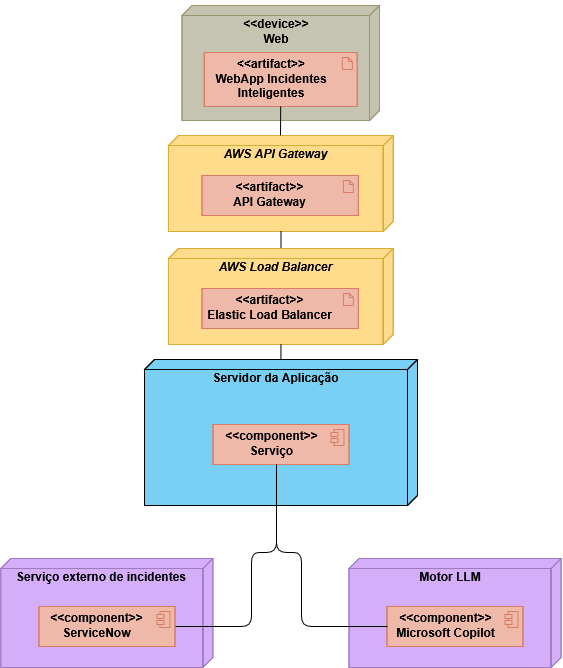
\includegraphics[width=110mm,keepaspectratio]{img/diagramaDeployment_v2}
		\caption[Diagrama de Implantação]{Diagrama de Implantação}
		\label{fig:deployDiagram}
	\end{figure}

%----------------------------------------------------------------------------------------
\section{Fluxo de Funcionamento}

	\todo{Rever}
	Um processo de consulta de incidentes (Figura \ref{fig:activityDiagram}), tem inicio no serviço a ser desenvolvido, onde, após a receção de um pedido de pesquisa, é realizada a consulta do incidente na plataforma externa de gestão de incidentes, assim como o histórico de tickets anteriores.
	
	De seguida, o serviço prepara a informação, combinando os dados do incidente atual com o histórico de incidentes anteriores, de forma a enriquecer o contexto disponível para análise e permitindo uma visão mais abrangente do problema. Já com os dados do incidente, é feita uma recolha dos eventos das aplicações, num período próximo ao da falha, e esses dados são adicionados à informação pré-processada do incidente.
	
	Após esta etapa de enriquecimento e agregação de dados, o fluxo é direcionado para o motor de modelos de linguagem de grande escala, responsável por duas tarefas principais. De forma paralela, o \gls{LLM} gera uma descrição do incidente em linguagem natural, tornando a informação técnica mais clara e acessível aos membros da equipa de suporte, e gera sugestões de mitigação priorizadas, com base no contexto do incidente, no histórico e nos eventos recolhidos, de forma a apoiar a tomada de decisão.
	
	Por fim, os resultados produzidos pelo motor de \gls{LLM} são novamente integrados no serviço central, que retorna ao utilizador a informação detalhada e contextualizada do incidente, incluindo a sumarização e as sugestões de mitigação.
	
	\begin{figure}[H]
		\centering
		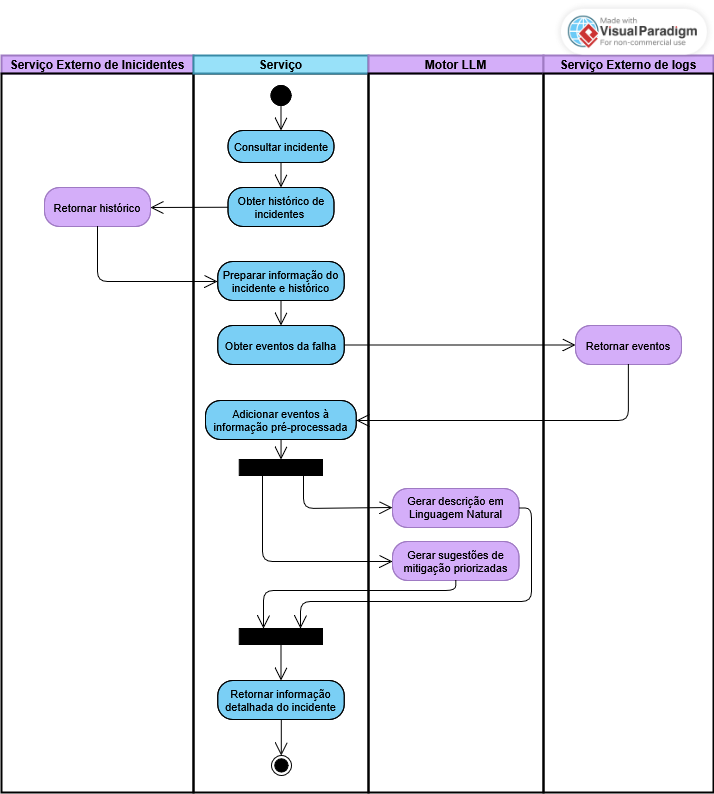
\includegraphics[width=\textwidth,keepaspectratio]{img/diagramaAtividade}
		\caption[Diagrama de Atividade]{Diagrama de Atividade}
		\label{fig:activityDiagram}
	\end{figure}

%	- Explicar o que acontece passo a passo, desde a criação de um incidente até ao apoio ao OCE.
%	- Sequência lógica do processo:
%		- Receção do incidente
%		- Análise inicial da descrição
%		- Consulta de incidentes semelhantes
%		- Consolidação de contexto
%		- Geração de apoio (resumo, sugestões, etc.)
%	- Onde entra o histórico
%	- Onde entram fontes adicionais
%	- Como o OCE interage com o sistema

%----------------------------------------------------------------------------------------
\section{Diagrama de Sequência}
	
	Apresenta-se apenas um diagrama de sequência que, representa um dos cenários de recuperação de contexto, especialmente útil para a analise de incidentes manuais. O diagrama descreve o fluxo seguido quando a pesquisa por incidentes históricos com o mesmo título não devolve resultados. Nesse caso, o sistema realiza uma segunda pesquisa, obtendo os incidentes (fechados e ativos) mais recentes da equipa em questão, de forma a encontrar outros problemas que possam estar relacionados com o incidente em análise. O diagrama na imagem \ref{fig:sequenceDiagram} permite visualizar a interação entre os principais componentes e compreender o comportamento da solução neste cenário.

	\begin{figure}[H]
		\centering
		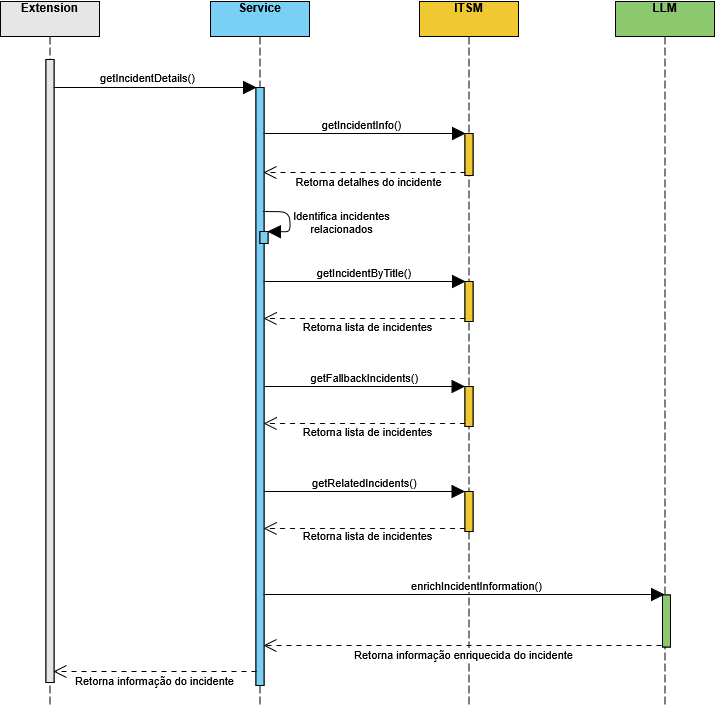
\includegraphics[width=\textwidth,keepaspectratio]{img/diagramaSequencia_v1}
		\caption[Diagrama de Sequência]{Diagrama de Sequência}
		\label{fig:sequenceDiagram}
	\end{figure}

%----------------------------------------------------------------------------------------
\section{Conclusão}

	\todo{TODO}